\chapter{Scanner}\label{chap:intro}

\section{Einleitung}
Aufgabe des Labors \textit{Systemnahes Programmieren} ist die Implementierung eines Compilers. Ein Compiler übersetzt ein Programm in einer vorgegebenen Sprache, in ein Programm in maschinennaher Sprache. Es sollen auch Fehler im Programmcode erkannt werden.

Die Aufgabe wurde in zwei Teilaufgaben aufgeteilt. Dieses Dokument befasst sich mit der ersten Teilaufgabe, der Implementierung eines Scanners.
Dabei handelt es sich um eine lexikalische Analyse, welche das vorgegebene Programm in Tokens, also ihre Grundsymbole, zerlegt.

Die Menge aller gültigen Zeichen und Bezeichner einer Programmiersprache ist üblicherweise eine reguläre Sprache.

Die gültigen Zeichen lauten wie folgt:
\begin{verbatim}
digit ::= 0 | 1 | 2 | 3 | 4 | 5 | 6 | 7 | 8 | 9
letter ::= A | B | C | … | Z | a | b | … | z
sign… ::= + | - | : | * | < | > | = | := | =:= | ! | && | ; | ( | ) | { | } | [ | ]
integer ::= digit digit*
identifier ::= letter (letter | digit)*
if ::= if | IF
while ::= while | WHILE
\end{verbatim}

Die gültigen Symbole bilden die reguläre Sprache
\begin{verbatim}
L( sign+ | … | sign] | integer | identifier | if | while)
\end{verbatim}

Zu dieser Sprache wird ein Automat erstellt. Dieser akzeptiert die Sprache und befindet sich in einem Finalzustand, wenn ein Wort akzeptiert wird, oder in einem Nicht-Endzustand, wird ein Wort nicht akzeptiert.

Erkannte Identifier werden in einer Symboltabelle gespeichert. Das Token enthält neben einem Verweis darauf auch die Informationen Zeile, Spalte, Typ. Sollten Symbole außerhalb der Menge der gültigen Zeichen oder Bezeichner gefunden werden, wird ein Fehlertoken erstellt.


\subsection{Voraussetzungen}
Um unser Projekt korrekt kompilieren zu können, sind einige Programme notwendig, die an dieser Stelle genannt werden sollen.
\begin{itemize}
  \item Gcc
  \item Make
  \item CMake (Version >= \textsc{3.5})
  \item Git
\end{itemize}

Möchte man diese Dokumentation generieren, benötigt man zudem
\begin{itemize}
  \item XeLaTeX
  \item BibTeX
  \item Python3
\end{itemize}
Das gesamte Projekt wurde mit Linux Mint 18 (Mate) getestet. Da eine Anforderung war, dass das Projekt mit Eclipse eingesetzt werden soll, haben wir beschlossen Eclipse Neon in der Version 4.6.3 zu nutzen, welches das Eclipse CDT Plugin in der Version 9.2.1 zur Entwicklung von C++ Programmen einsetzt.

Erstellen eines Projekts
Um das Projekt korrekt in Eclipse zu importieren, muss das Projekt zuerst geladen werden. Wir haben uns dazu entschieden, Github als Host unserers Git Repositories zu nutzen.

Das Projekt kann man wie folgt laden:

\begin{lstlisting}[language=bash,numbers=none]
git clone https://github.com/TobsCore/sysprog.git
\end{lstlisting}

Man erkennt, dass ein neues Verzeichnis mit dem Namen \texttt{sysprog/} erstellt wurde. Dies ist unser Projekt-Verzeichnis. Wie das Projekt organisiert ist, wird genauer in~\ref{sec:orga_code} genauer beleuchtet.

Es handelt sich bei uns um ein \textit{CMake Projekt}, was man unter anderem daran erkennt, dass sich im Hauptverzeichnis die Datei \texttt{CMakeLists.txt} befindet. Diese Datei wird dazu genutzt, dass alle Programmteile korrekt gelinkt werden und man kann dort verschiedene \textit{Compile Targets} definieren. Was dies bedeutet, werden wir sehen, wenn das Projekt erfolgreich in Eclipse importiert wurde.

Da Eclipse jedoch nicht mit CMake Projekten umgehen kann, kann man sich ein Eclipse Projekt durch CMake generieren lassen. Um diesen Schritt zu vereinfachen, haben wir ein kleines Script geschrieben, welches sich im \texttt{sysprog/} Verzeichnis befindet und dort ausgeführt werden kann.

\lstinputlisting[language=bash,numbers=none,caption=Das Init Eclipse Script]{../init_eclipse.sh}

An dieser Stelle sei anzumerken, dass sich in unserem Projekt 2 unterschiedlicheCMakeLists.txt Dateien befinden.
\begin{verbatim}
sysprog/CMakeLists.txt
sysprog/src/CMakeLists.txt
\end{verbatim}

Diese Dateien haben beinahe den selben Inhalt, was den Grund hat, dass wir das Programm auch unter MacOS mit CLion entwickeln wollten und Eclipse nicht damit umgehen kann, dass der Ordner \texttt{cmake-build-debug/}, in den die Executables geschrieben werden im Quellcodeverzeichnis liegt. Die \texttt{CMakeLists.txt} Datei, die zur Generierung des Eclipse Projekts genutzt wird, liegt also in \texttt{
sysprog/src/CMakeLists.txt}.

\subsection{Generierung des Eclipse Projekts}
Es wurde ja bereits beschrieben, das das Projekt in ein Eclipse Projekt umwandelt. Dieses Script kann man einfach per

\begin{lstlisting}[language=bash,numbers=none]
./init_eclipse.sh
\end{lstlisting}

aufrufen. Hierbei wird der Ordner \texttt{cmake-build-debug/} generiert, in den dann die Executables nach erfolgreichem Kompilieren landen.

Das Projekt kann nun in Eclipse eingebunden werden. Hierzu wählt man \textit{File} -> \textit{Import}. Unter \textit{General} wählt man dann den Eintrag \textit{Existing Projects into Workspace}.
Bei dem Punkt \textit{Select root directory} wählt man dann den gerade generierten Ordner \texttt{sysprog/cmake-build-debug/}.

Das Ganze sollte dann wie auf Bild~\ref{fig:import_project} aussehen. Wichtig ist hierbei, dass die Option \textit{Copy projects into workspace} deaktiviert ist.

\begin{figure}[!htb]
    \centering
      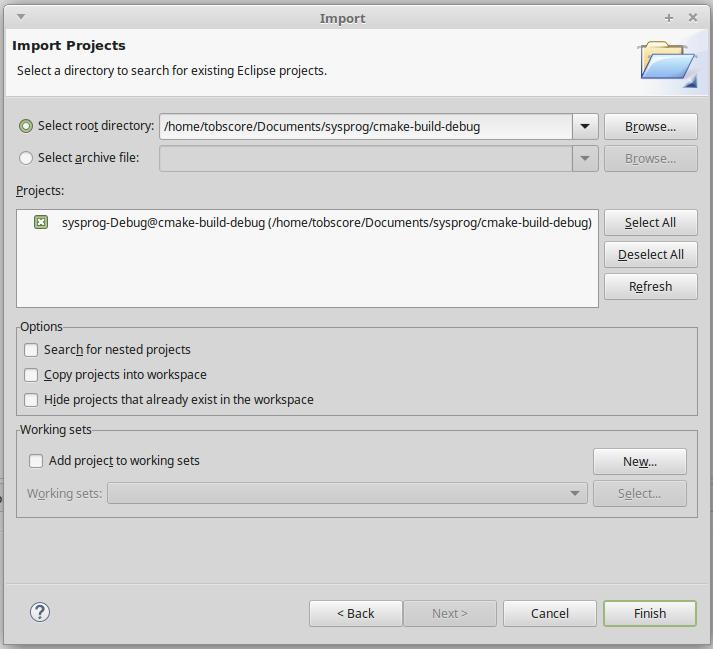
\includegraphics[width=0.6\linewidth]{Import_Project.jpg}
    \caption{Import Dialog}\label{fig:import_project}
\end{figure}

Durch das Klicken auf \textit{Finish} sollte das Projekt dann korrekt eingebunden sein.
\clearpage

\setlength{\intextsep}{-20pt}%
\begin{wrapfigure}{r}{0.35\textwidth}
  \centering
    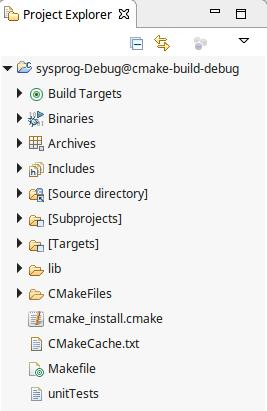
\includegraphics[width=0.32\textwidth]{Project_Structure.jpg}
    \caption{Die Projekt\-struktur in Eclipse}\label{fig:project_structure}
\end{wrapfigure}

In Bild~\ref{fig:project_structure} kann man dann sehen, wie die Projektstruktur in Eclipse aussieht.

Unter \textit{Build Targets} kann man dann den Eintrag \texttt{[exe] sysprogMain} auswählen und bauen, indem man einen Rechtsklick machet und \textit{Build Target} auswählt. Möchte man die Unit Tests laufen lassen, so kann man diese über \texttt{[exe] unitTests} kompilieren. Im Project Explorer wird dann unter Binaries das ausführbare Programm erstelllt.


Ausführen lassen sich die Programme direkt aus Eclipse über einen Rechtsklick auf eines der Binaries und danach durch Auswählen von \textit{Run As} -> \textit{Local C/C++ Application}.

Wie man erkennen kann, werden die Tests ausgeführt und in der Konsole innerhalb von Eclipse ausgegeben. Man kann dann auch Programmparameter für das Binary festlegen und somit auch das Hauptprogramm korrekt starten.

\subsection{Projekt ohne Eclipse kompilieren}
Möchte man das Projekt zum Laufen bringen, ohne sich an Eclipse binden zu müssen, so reicht es ein neues Verzeichnis zu erstellen, in dem dann durch CMake ein Makefile generiert wird. Dieses kann man dann sehr einfach ansprechen um BuildTargets zu bauen. Dies wird wie folgt gemacht.

\begin{lstlisting}[language=bash,numbers=none]
mkdir cmake-build-debug
cd cmake-build-debug
cmake ..
make all
\end{lstlisting}

Es lassen sich die Build Targets \texttt{sysprogMain} und \texttt{unitTests} auch gezielt bauen, durch den Aufruf

\begin{lstlisting}[language=bash,numbers=none]
make sysprogMain
make unitTests
\end{lstlisting}

In diesem Ordner werden dann die Binaries gebaut, die dann ausgeführt werden können.
\begin{lstlisting}[language=bash,numbers=none]
make unitTests
./unitTests
\end{lstlisting}

\subsection{Organisation des Codes}\label{sec:orga_code}
Wenn man das Repository herunter geladen hat, so findet man 2 Verzeichnisse. In \texttt{Documentation/} befindet sich diese Dokumentation, die mit \XeLaTeX\ erstellt wurde. Hat man \texttt{Python3} installiert, so kann man diese Dokumentation ganz einfach über \texttt{make} generieren lassen.

Das \texttt{src/} Verzeichnis enthält den Code für unser Programm, die Tests und alles was man zum erfolgreichen Bauen benötigt.

In dem \texttt{lib/} Verzeichnis befindet sich die \textit{Google Test} Bibliothek, welche wir verwendet haben um unsere Unit Tests zu schreiben.

Die Unit Tests sind im Verzeichnis \texttt{test/}, wobei dort einige Testdateien im Verzeichnis \texttt{testData/} liegen. In dieser Ausarbeitung soll jedoch nicht näher auf die Tests eingegangen werden, da das Resultat zum Testen benutzt werden kann.

Der eigentlich Source Code liegt dann unter \texttt{main/}.
